\documentclass[11pt]{article}

\newcommand{\cnum}{CM146}
\newcommand{\ced}{Winter 2018}
\newcommand{\ctitle}[3]{\title{\vspace{-0.5in}\cnum, \ced\\Problem Set #1: #2}}

\newcommand{\solution}[1]{{{\color{blue}{\bf Solution:} {#1}}}}
\usepackage[usenames,dvipsnames,svgnames,table,hyperref]{xcolor}
\usepackage{amsmath}
\usepackage{graphicx}
\graphicspath{ {images/} }
\renewcommand*{\theenumi}{\alph{enumi}}
\renewcommand*\labelenumi{(\theenumi)}
\renewcommand*{\theenumii}{\roman{enumii}}
\renewcommand*\labelenumii{\theenumii.}


\begin{document}
\ctitle{3}{Atibhav Mittal (ID: 804598987)}
\author{}
\date{}
\maketitle
\vspace{-0.75in}

\section{Problem 1}
\begin{enumerate}
\item Problem 1a
\solution{} \newline
The VC dimension of the given function is 3
The following images show that for any labeling of 3 points, we can find a 
decision boundary that belongs to the class of functions: $ax^2 + bx + c$ \newline
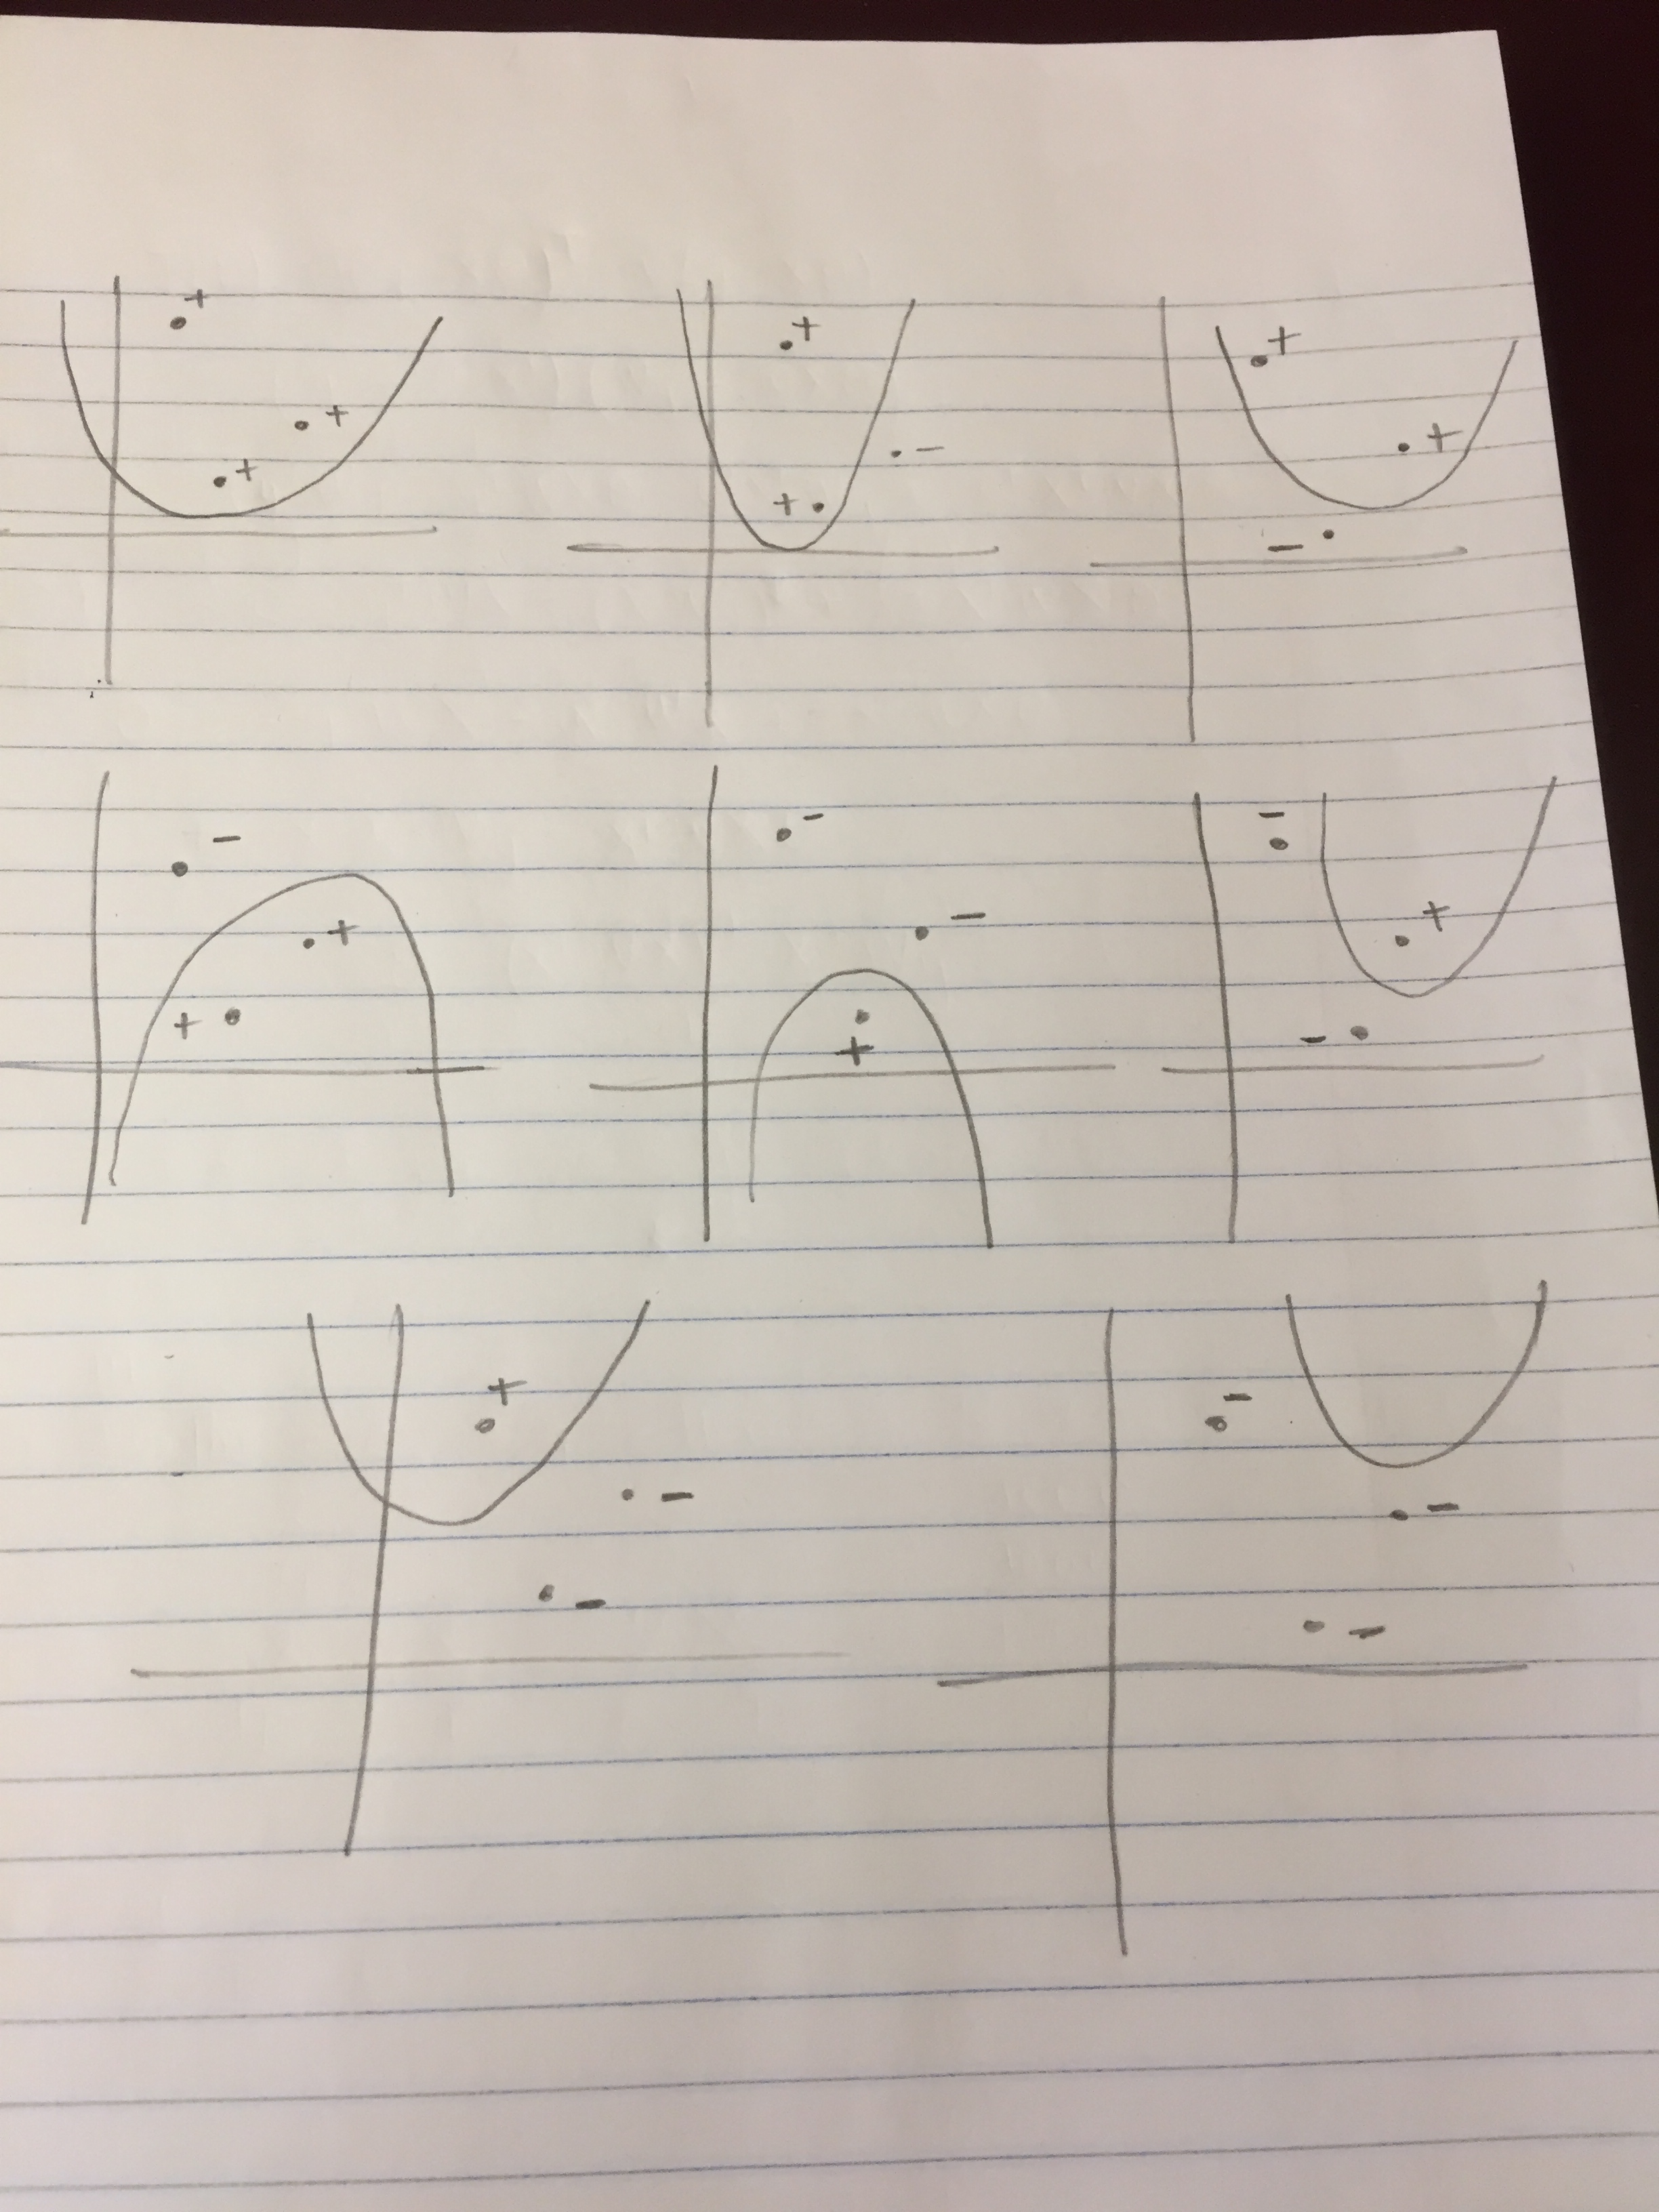
\includegraphics[scale=0.1]{prob_1.JPG} \newline
This means that VC dimension $\geq 3$ \newline
However, consider 4 points given to us. Out of these 4 points, one point 
will have the largest x-axis value, one will have the smallest x-axis value,
one will have the largest y-axis value and one will have the smallest y-axis value.
Since the function only finds decision boundaries that are either upward
or downward facing parabolas, a labeling where the points with the following labelling
cannot be satisfied
\begin{enumerate}
\item largest x-value point: +
\item smallest x-value point: +
\item largest y-value point: -
\item smallest y-value point: -
\end{enumerate}

Hence, VC dimension $<$ 4 and VC Dimension $\geq 3$ \newline
Thus, VC dimension = 3 

\end{enumerate}

\newpage
\section{Problem 2}

\solution{} \newline
Assume that $x = \begin{bmatrix}
x_1 \\
x_2
\end{bmatrix}
$ and $ z = \begin{bmatrix}
z_1 \\
z_2
\end{bmatrix}
$
$$
K_\beta (x, z) = (1 + \beta x \cdot z)^3
$$
\begin{align*}
K_\beta (x, z) = & x_1^3 \beta^3 z_1^3 + x_2^3 \beta^3 z_2^3 + 3 x_1 x_2^2 \beta^3 z_1 z_2^2 + 3 x_1^2 x_2 \beta^3 z_1^2 z_2 + 3 x_1^2 \beta^2 z_1^2 + 3 x_2^2 \beta^2 z_2^2 + \\ 
&  6 x_1 x_2 \beta^2 z_1 z_2 + 3 x_1 \beta z_1 + 3 x_2 \beta z_2 + 1
\end{align*}
$$
\Rightarrow \phi_{\beta}(\boldsymbol{x}) = 
\begingroup
\renewcommand*{\arraystretch}{1.5}
\begin{bmatrix}
1 \\
\sqrt{3}\sqrt{\beta}x_1 \\ 
\sqrt{3}\sqrt{\beta}x_2 \\
\sqrt{6} \beta x_1 x_2 \\
\sqrt{3} \beta x_1^2 \\
\sqrt{3} \beta x_2^2 \\
\sqrt{3}\beta^{3/2} x_1^2 x_2 \\
\sqrt{3}\beta^{3/2} x_1 x_2^2 \\
\beta^{3/2}x_1^3 \\
\beta^{3/2}x_2^3 \\
\end{bmatrix}
\endgroup
$$
The kernel function $K_{\beta}$ is similar to the $K(x,z) = (1 + x\cdot z)^3$, when $\beta=1$
The only similarity when $\beta \neq 1$, is the constant 1, which is the first feature of this
higher dimensional space. \newline
The role of beta is to provide a weighing factor. The beta factor, scales each feature differently,
as shown above. For richer/more complex features, if $\beta > 1$, it weighs the higher order
features more in the kernel, and thus they have a larger contribution in the inner product.
If $\beta < 1$, it weighs the lower order features more, and the higher order features less.
If $\beta = 1$, it weighs all the features in the kernel equally. 

\newpage
\section{Problem 3}
\begin{enumerate}
\item 
\solution{} \newline
Consider $w = \begin{bmatrix}
w_1 \\
w_2
\end{bmatrix}$
$$
w^T x_1 = w_1 + w_2
$$
$$
w^T x_2 = w_1
$$
Using the values of the labels, we get the inequalities:
$$
w_1 + w_2 \geq 1
$$
$$
w_1 \leq -1 \Rightarrow w_1^2 \geq 1
$$
$$
w_2 \geq 2 \Rightarrow w_2^2 \geq 4
$$
Since we're trying to minimize $\frac{1}{2} ||w||^2$, we can instead
minimize $w_1^2 + w_2^2$
Hence, $w_1 = -1, w_2 = 2$
$$
w^* = \begin{bmatrix}
-1 \\
2
\end{bmatrix}
$$
\item 
\solution{} \newline
If we allow a non-zero offset, the best separation would pass through the center,
and the projection from each of the lines to the separating hyperplane would be
perpendicular to it. This corresponds to:
$$
w^* = \begin{bmatrix}
0 \\
2
\end{bmatrix}, b^* = -1
$$
\end{enumerate}

\newpage
\section{Problem 4}
\subsection{}
\begin{enumerate}
\setcounter{enumi}{3}
\item \solution{} \newline
The number of unique words in the dataset is 1811. \newline
Hence, the dimensionality of the dataset is 1811.
\end{enumerate}
\subsection{}
\begin{enumerate}
\setcounter{enumi}{1}
\item Its beneficial to maintain class proportions across folds, because this
	gives us a better picture of the actual dataset in the sense that the actual
	proportions of the dataset are reflected. This enables us to have a model that
	generalizes well.
\setcounter{enumi}{3}
\item \solution{} \newline
\begin{center}
\begingroup
\def\arraystretch{1.5}
\begin{tabular}{ c | c | c | c }
C & accuracy & F1-score & AUROC \\
\hline
$10^{-3}$ & 0.7089 & 0.8297 & 0.8105 \\
$10^{-2}$ & 0.7107 & 0.8306 & 0.8111 \\
$10^{-1}$ & 0.8060 & 0.8755 & 0.8575 \\
$10^{0}$ & 0.8146 & 0.8749 & 0.8712 \\
$10^{1}$ & 0.8182 & 0.8766 & 0.8696 \\
$10^{2}$ & 0.8182 & 0.8766 & 0.8696 \\
\hline
best C & 10 & 10 & 1
\end{tabular}
\endgroup
\end{center}
For the accuracy measurement, we can see that the performance improves as C increases. However,
we can see that it slowly approaches the value 0.8182, and will probably not increase much for
larger C, and will probably decrease for more C. \newline
For the F1-Score measurement, the C value continues to increase till C = 10, and then becomes
fairly constant, similar to the accuracy measurement. However, the performance according to this
metric is better than the performance measured using accuracy. (This does not say anything about 
which metric is better though). \newline
For the AUROC metric, the C value first increases till C=1, and then decreases after that. The
performance measured is comparable to the performance measured using F1-score. \newline 
\end{enumerate}

\subsection{}
\begin{enumerate}
\item From the above results, we choose the following c values:
\begin{enumerate}
\item Accuracy: C = 10
\item F1-Score: C = 10
\item AUROC: C = 1
\end{enumerate}

\setcounter{enumi}{2}
\item The results on the test set are as follows:
\begin{enumerate}
\item Accuracy: 0.7429
\item F1-Score: 0.4375
\item AUROC: 0.7405
\end{enumerate}
\end{enumerate}
\end{document}
